\chapter{Preparing a high-quality PDF from LaTeX}\label{sec:PDFprep}
If the author chooses to complete the publications process using LaTeX\, the author must incorporate feedback and edits in to the LaTeX source files and prepare the final PDF, following these guidelines.

\section{PDF tagging}\label{sec:PDFtagging}
PDF tagging is a process whereby the components of the PDF document (headings, figures, tables, text) are marked so that a document reader can understand the document. This is useful when text to speech converters are being used. The process of tagging is also known as structuring, so that a tagged document might also be referred to as a structured document\footnote{This is a test}.

LaTeX does not prepare a tagged PDF document. The current solution to this is to use the tagging capability built in to Adobe's Acrobat Pro.

%To prepare a tagged document, follow these steps:
%\begin{enumerate}
%\item Add tags. Go to the `Advanced' menu. Select `Accessibility', then `Add tags to document'.
%\item Add alternative text for figures. Context-click the Figure, select `Properties', and fill in `Alternate Text'. Alternatively, try the process outlined below.
%\item Specify the document language. Go to the `File' menu. Select `Document Properties', then the `Advanced' tab, `Language' field. In some versions of Acrobat, the sequence is `File', `Properties', `Reading Options', `Language'.
%\item Define tab order.
%\begin{enumerate}
%\item Go to the `View' menu. Select `Navigation tabs', then `Pages'.
%\item Click on any page, then type Ctrl-A (or Command-A on a Mac) to select all the pages.
%\item Go to the `Options' menu in the top right of the dialog box, and select `Page Properties'
%\item In the `Tab Order' tab, select `Use document structure'.
%\end{enumerate}
%\item Make sure tables have headings. 
%\begin{enumerate}
%\item Go to the `View' menu. Select `Navigation tabs', then `Tags'.
%\item Select the `Tags' tab. This panel shows the document structure as a tree.
%\item Navigate to the table cells that should be headers.
%\item Check they have the type <TH>. If not, then right click on the header cell, select `properties', select the `Tag' tab, and change the value for `Type' to <TH>.
%\end{enumerate}
%\item Make sure all Chapters (or sections, if there are no chapters in the document) are correctly tagged.
%\end{enumerate}
%
%\section{Alt-text on images and equations}
%`Alt text' is a textual description of an equation, link or figure. The following short equation should pop-up some text when a user passes a mouse over it. This should work in most PDF readers:
%\begin{equation}
%\pdftooltip{a^2+b^2=c^2}{An equation}
%%a^2+b^2=c^2
%\end{equation}
%
%The alt text can be added after the PDF is compiled, or written in to the source document. The rest of this section describes how it can be added to the source and generated by LaTeX using the \href{pdfcomment}{http://www.ctan.org/pkg/pdfcomment} package. The general form of the command is:
%
%\begin{verbatim}
%\pdftooltip{<item>}{<pop-up text>}
%\end{verbatim}
%
%The previous equation was generated using this code:
%
%\begin{verbatim}
%\begin{equation}
%\pdftooltip{a^2+b^2=c^2}{An equation}
%\end{equation}
%\end{verbatim}
%
%The same approach can be used to create alt-text for images. For example, Figure \ref{fig:NRELimagesWithAltText} has been labeled. The code for this image is:
%
%\begin{verbatim}
%\begin{figure}[!h]
%\centering
%\hfill
%\subfigure[Wind turbines at the Forward Wind Energy Center in Fond du Lac and Dodge Counties, Wisconsin. (Photo by Ruth Baranowski / NREL)] {\pdftooltip{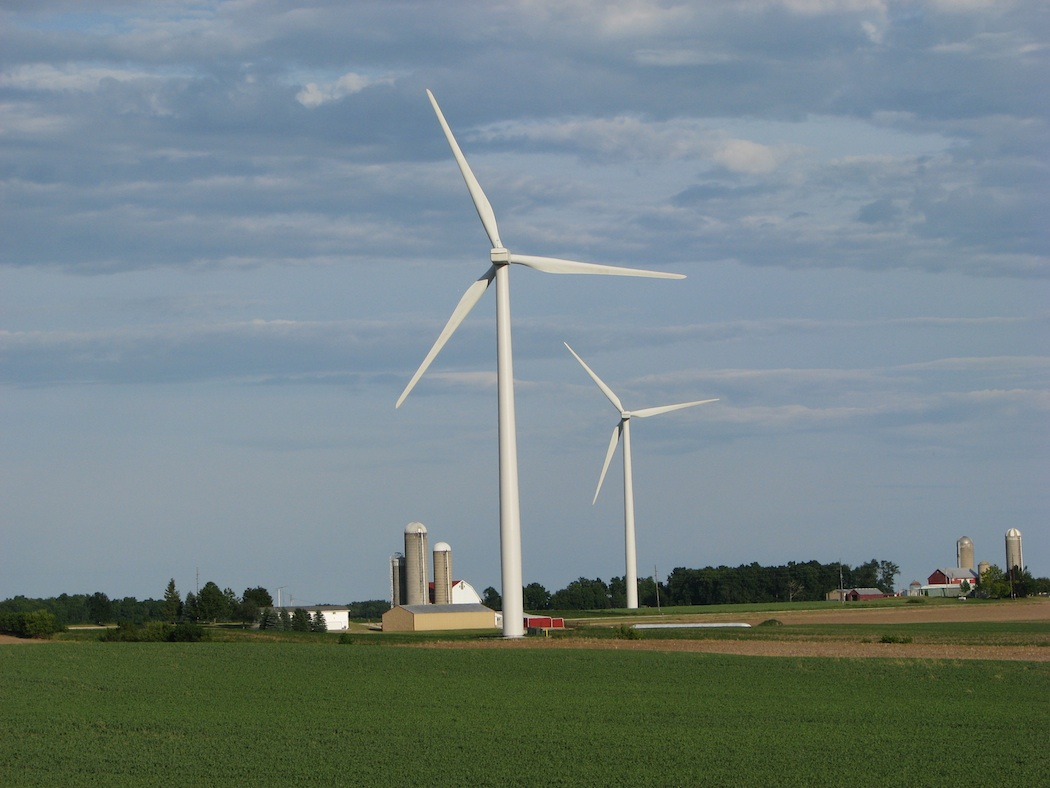
\includegraphics[height=2.5in]{files/21206}}{This is an image}}
%~ 
%\hfill
%\subfigure[Aerial view of the National Wind Technology Center.  (Photo by Dennis Schroeder / NREL)] {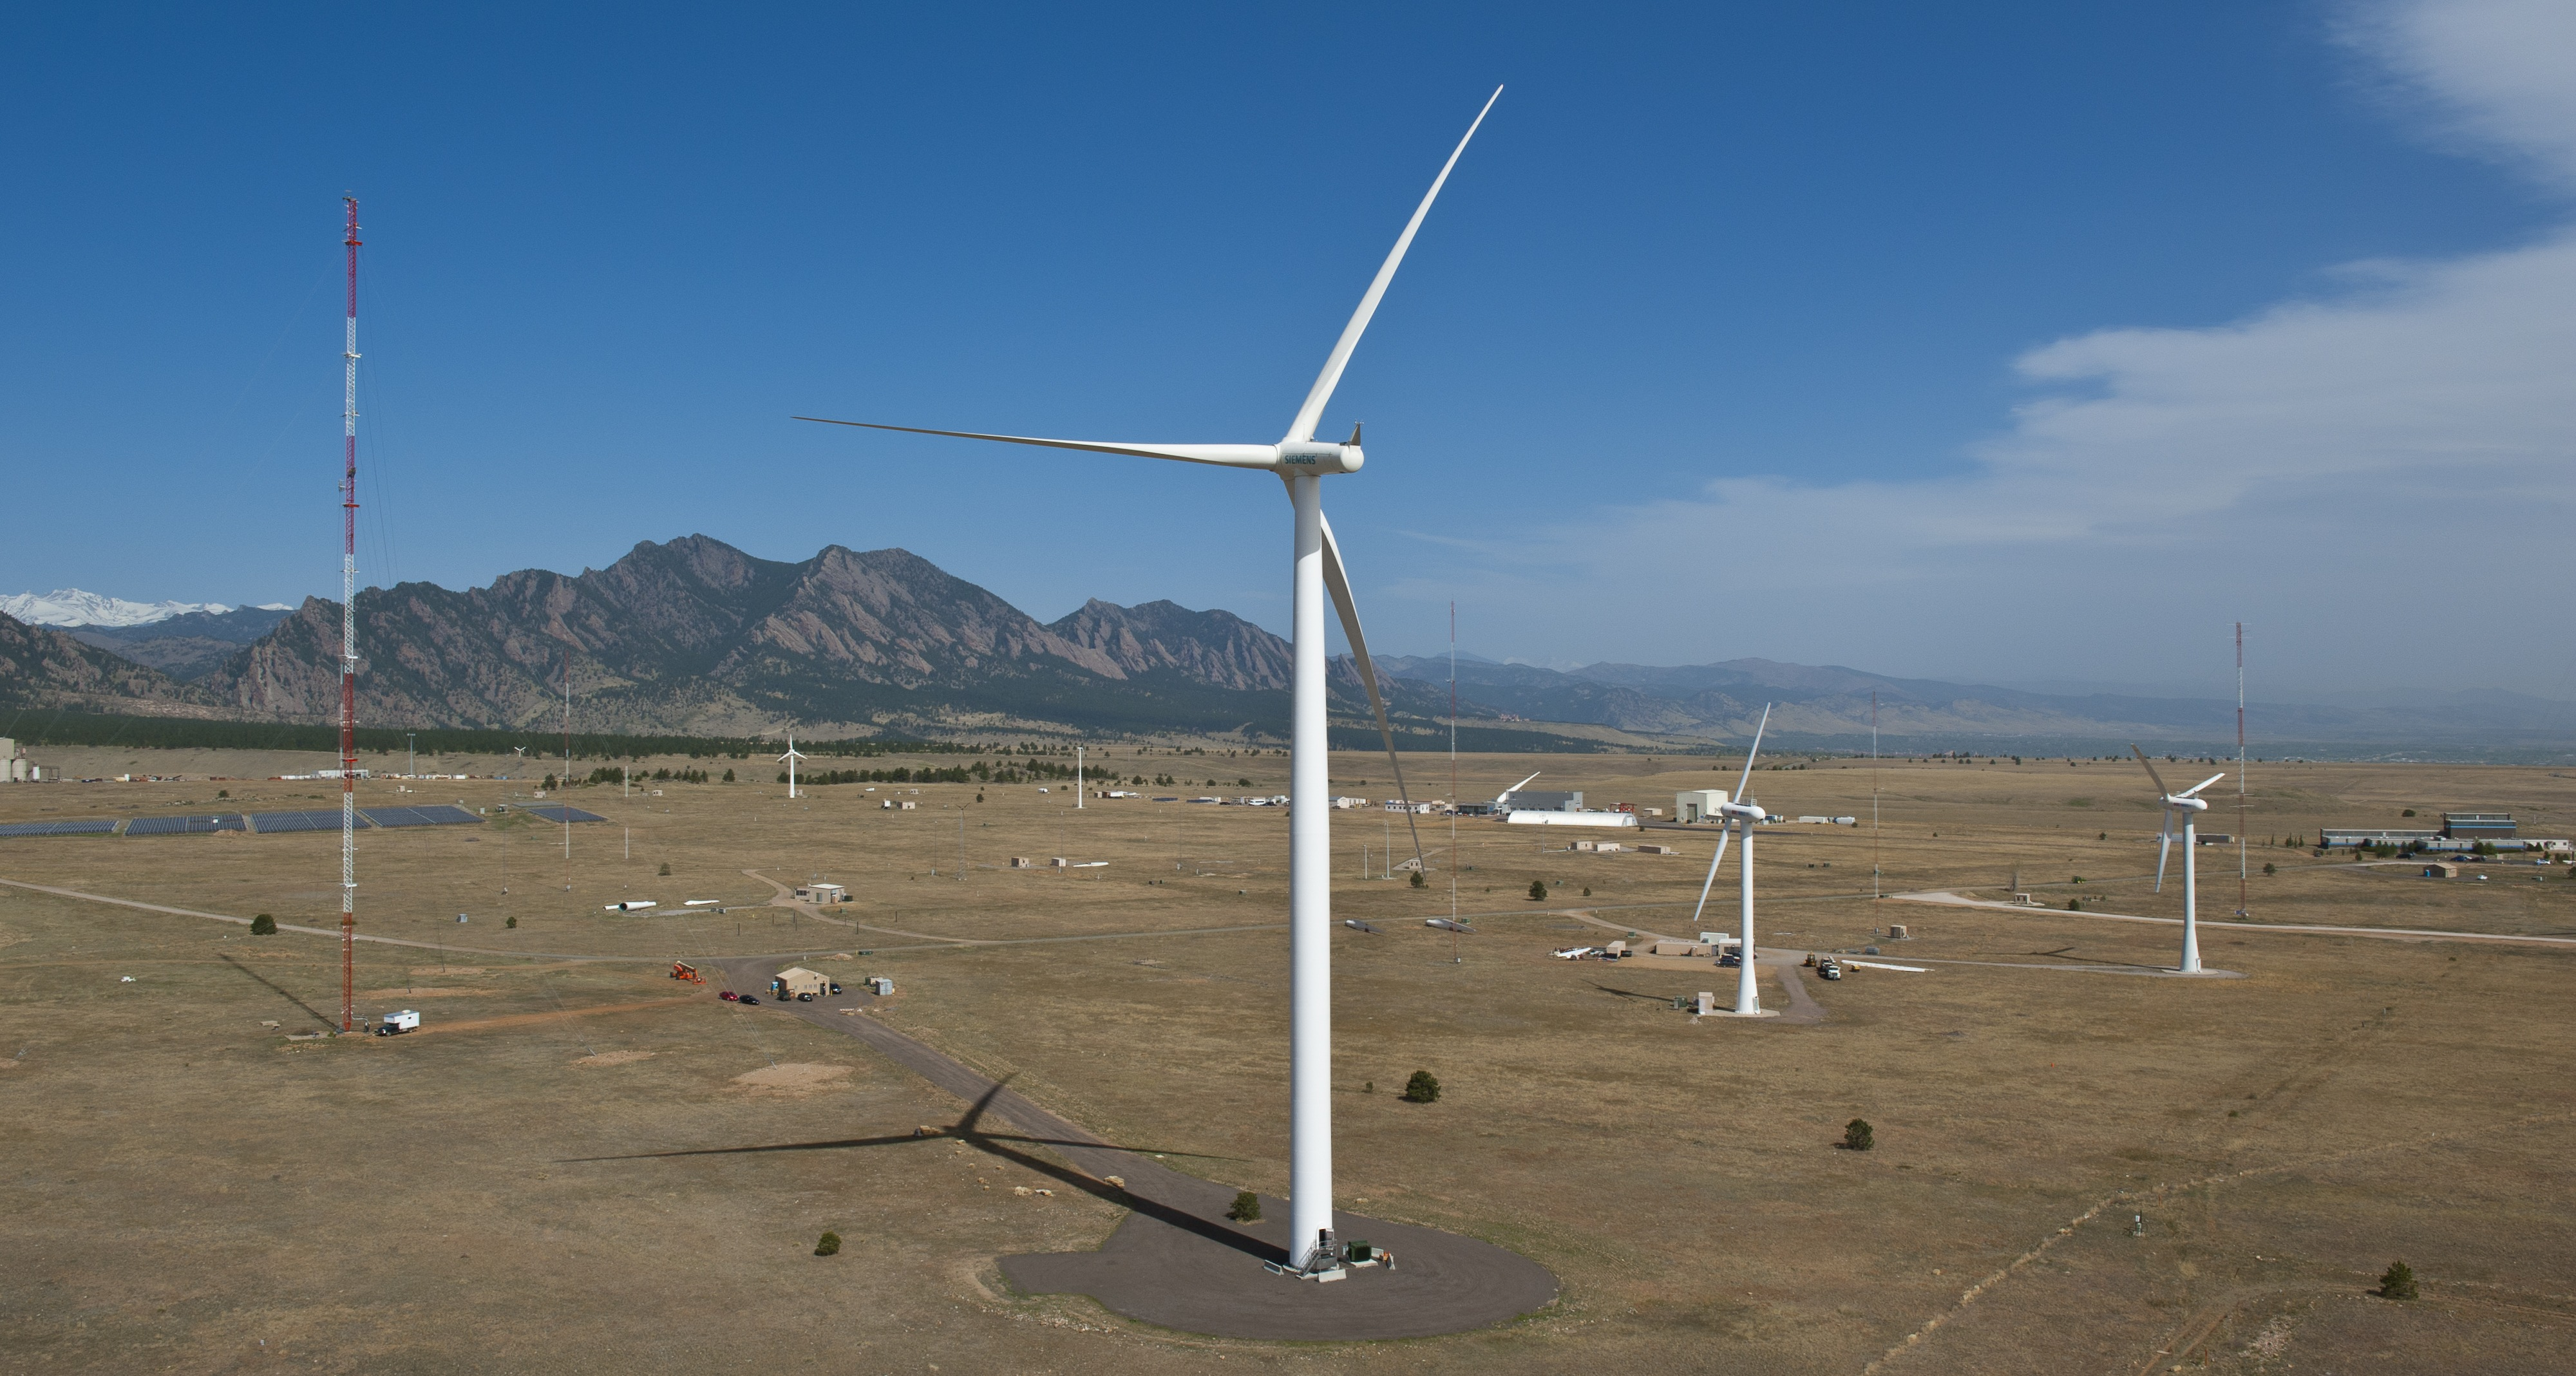
\includegraphics[height=2.5in]{files/20018}}
%\hfill
%\caption{NREL images}\label{fig:NRELimagesWithAltText}
%\end{figure}
%\end{verbatim}
%
%\begin{figure}[!h]
%\centering
%\hfill
%\subfigure[Wind turbines at the Forward Wind Energy Center in Fond du Lac and Dodge Counties, Wisconsin. (Photo by Ruth Baranowski / NREL)]{\pdftooltip{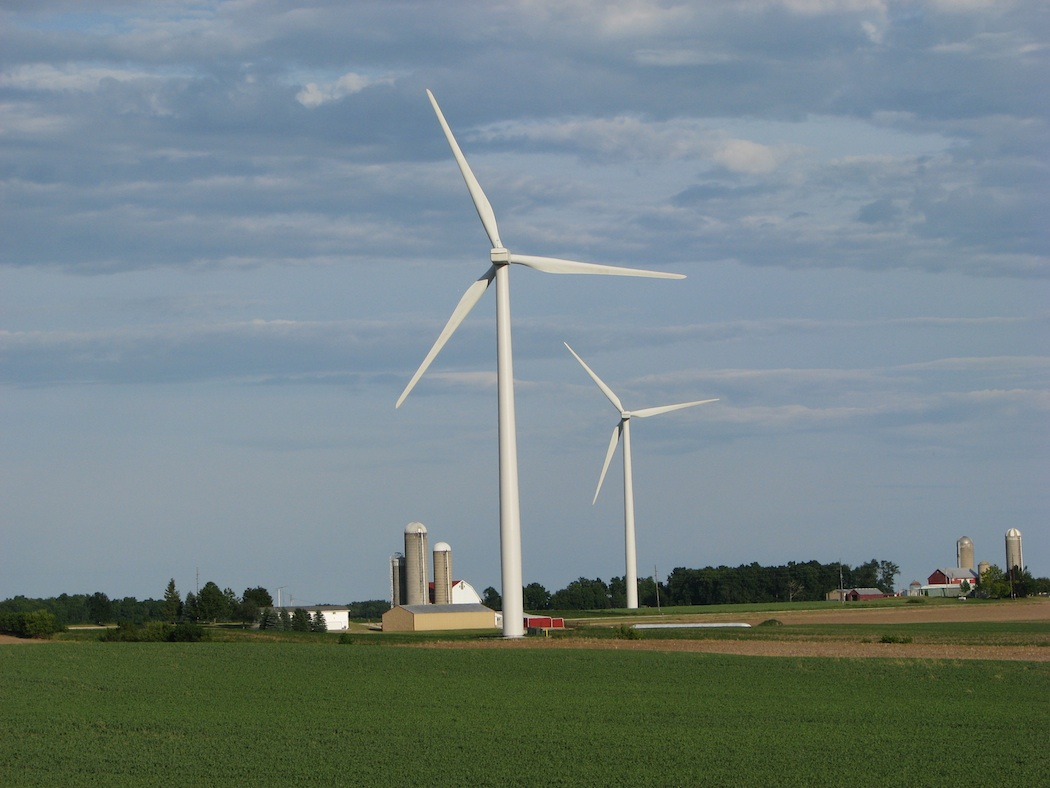
\includegraphics[height=2.5in]{files/21206}}{This is an image. It may be possible to propagate the caption into this text.}}
%%{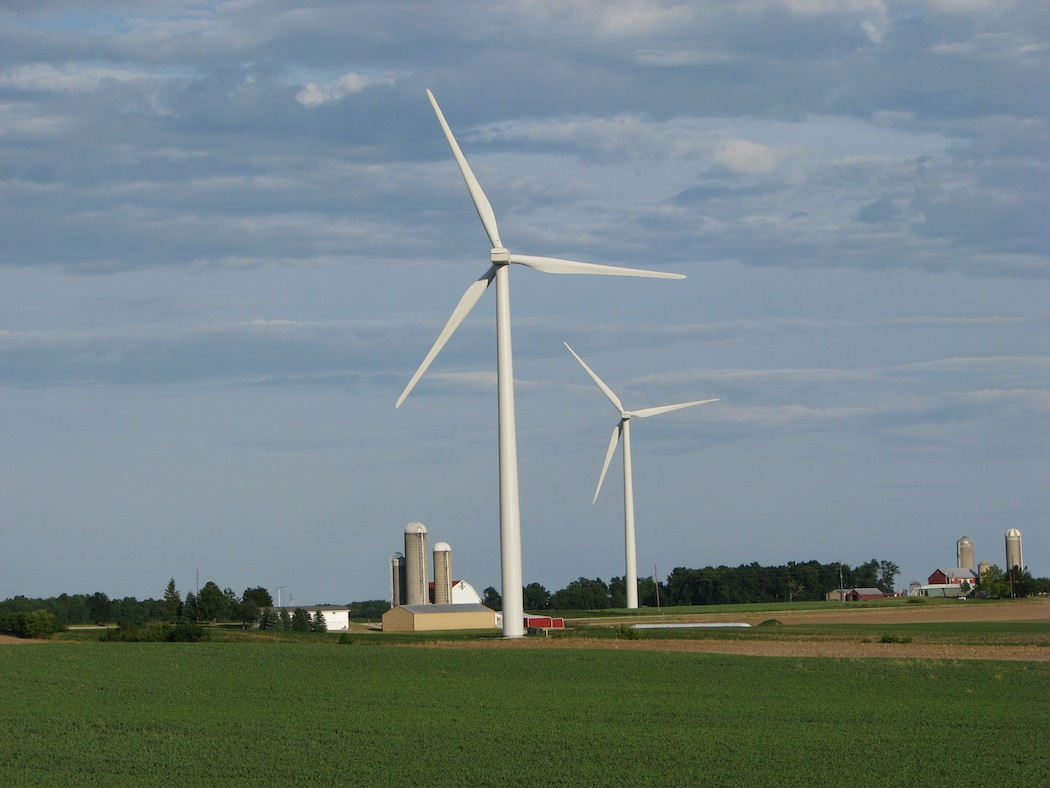
\includegraphics[height=2.5in]{21206}}
%~ %add desired spacing between images, e. g. ~, \quad, \qquad etc. (or a blank line to force the subfigure onto a new line)
%\hfill
%\subfigure[Aerial view of the National Wind Technology Center. (Photo by Dennis Schroeder / NREL)]{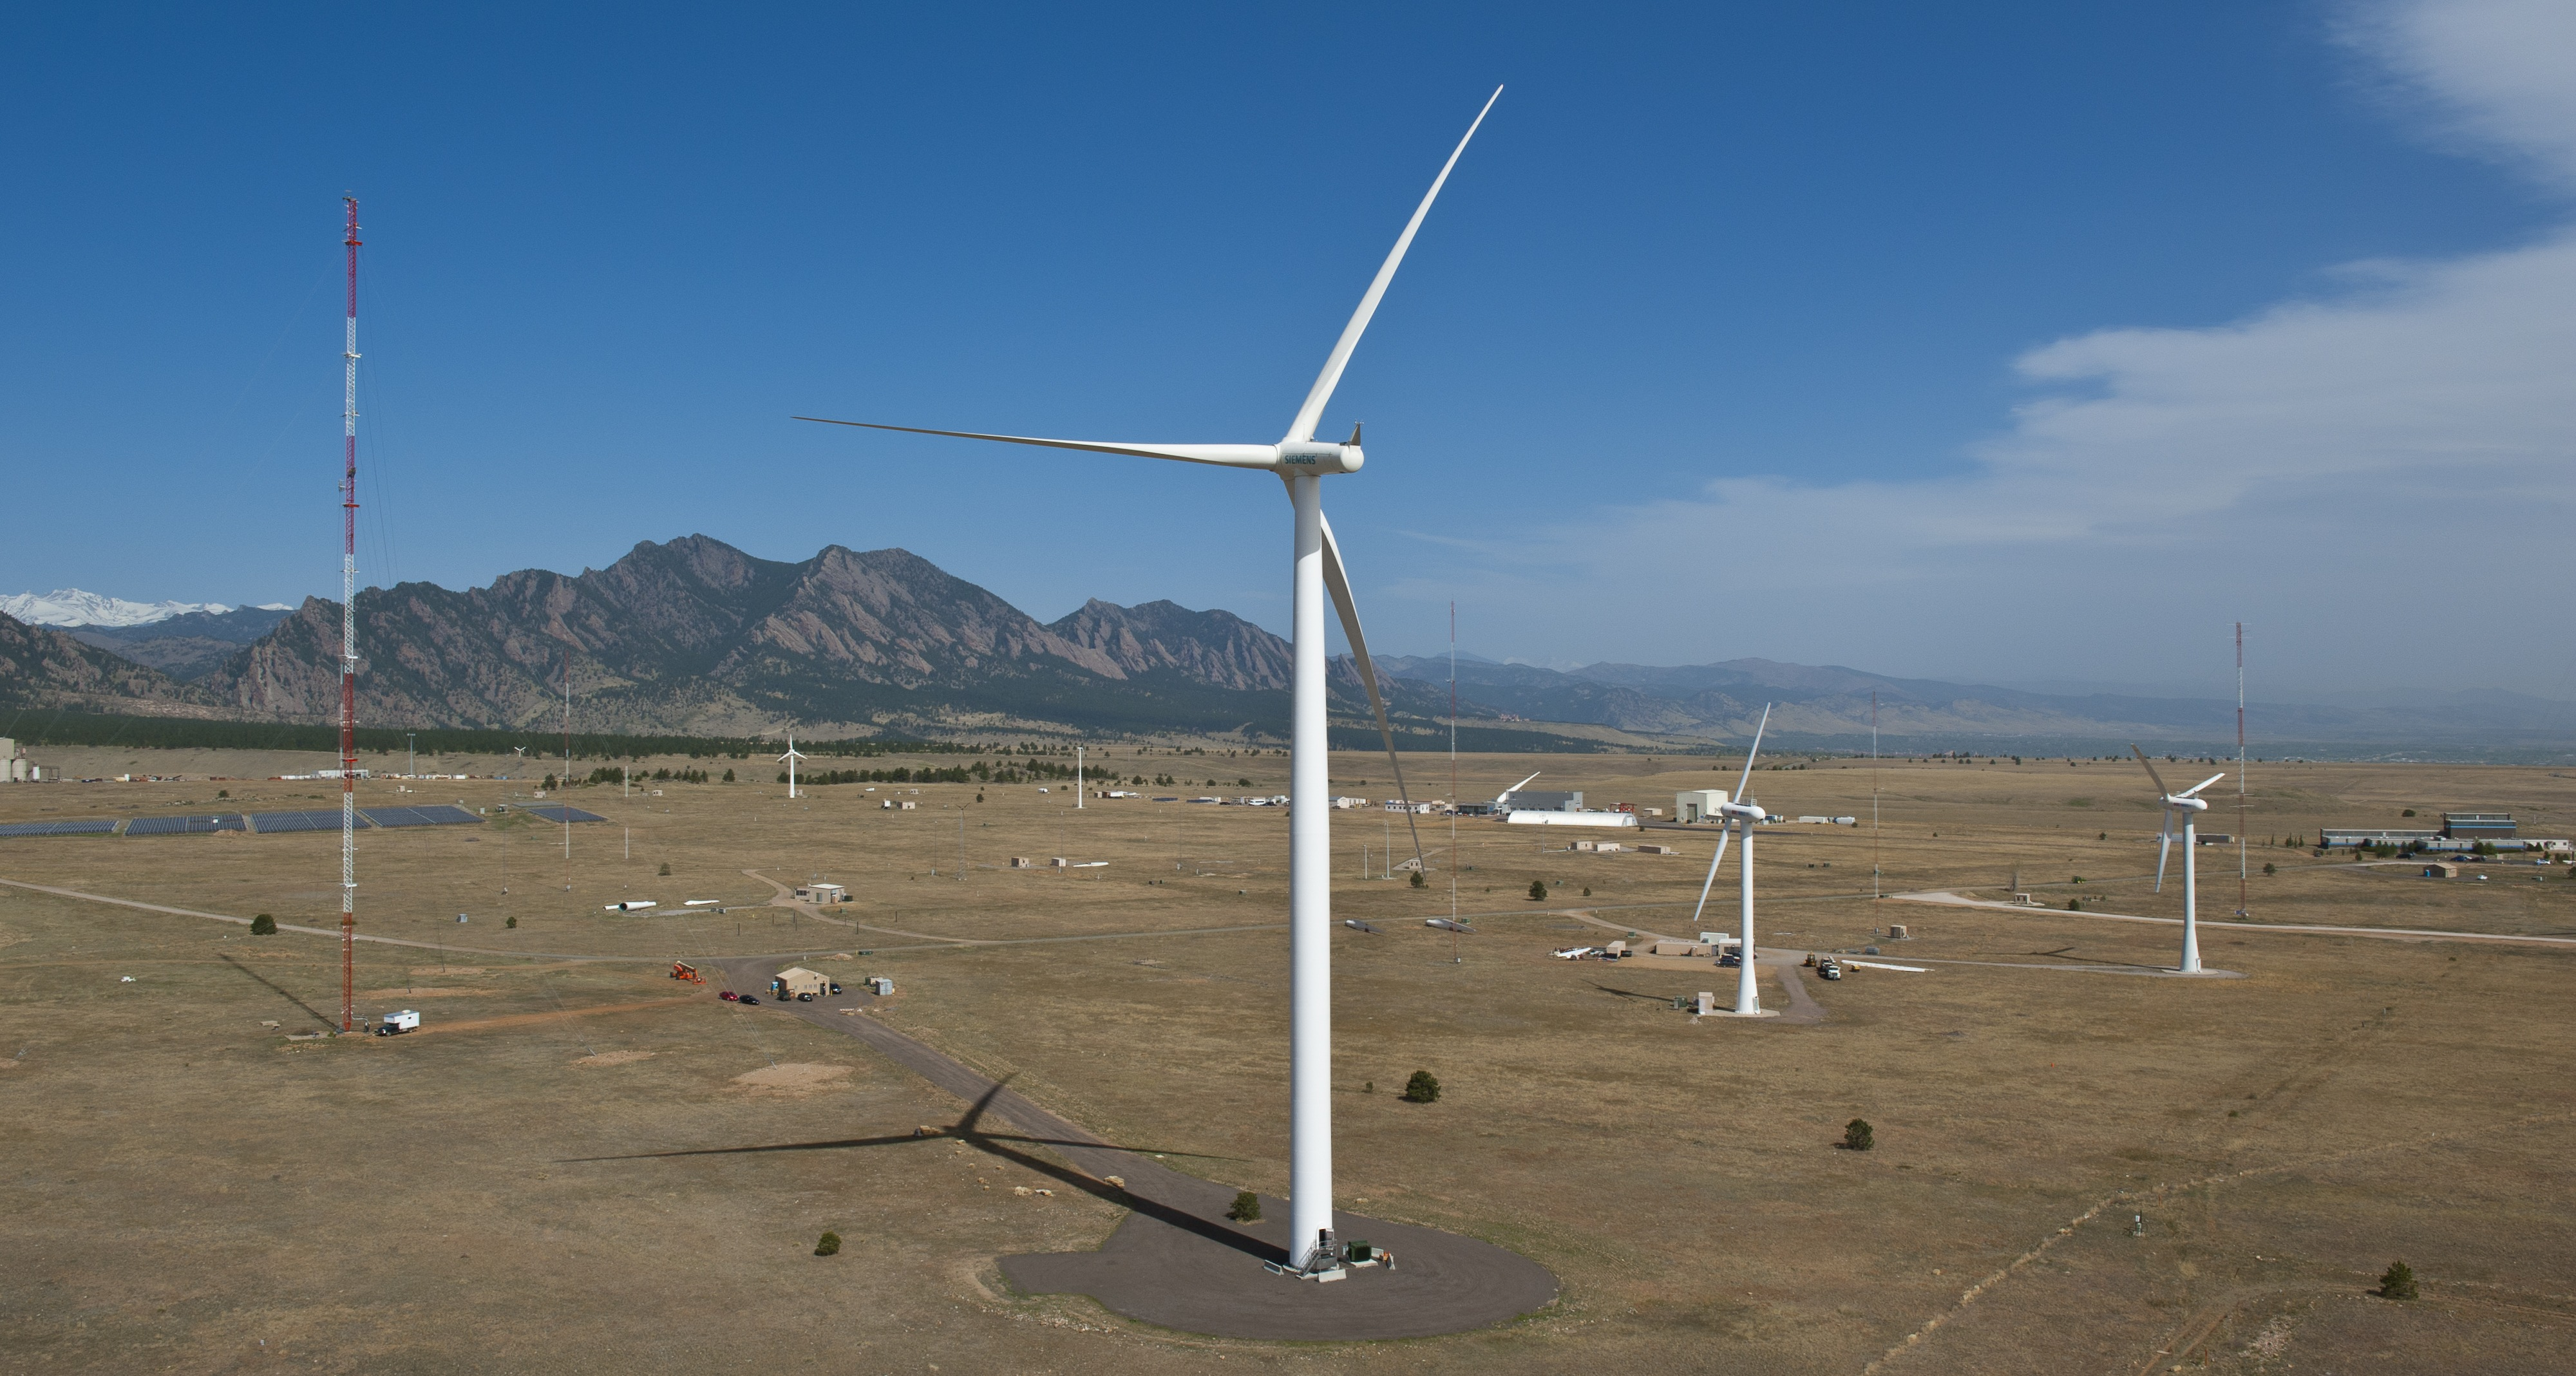
\includegraphics[height=2.5in]{files/20018}}
%\hfill
%\caption{NREL images with "alt text"}\label{fig:NRELimagesWithAltText}
%\end{figure}
%

\section{Embedded fonts}
NREL requires that all fonts be embedded in the the final PDF. Check the PDF for embedded fonts using a PDF viewer. For example, in Adobe Acrobat Reader, look at the `fonts' tag of the document properties. If any fonts are not shown as being an \emph{embedded subset}, try the conversion again. 

Encapsulated postscript figures are particularly prone to having undefined fonts. Check by compiling the document in draft mode, and seeing if the fonts are still present in the output PDF. To fix this problem, change \emph{.eps} files to \emph{.png} files. To do this `on the fly', use this in the document's preamble:

\begin{lstlisting}
\usepackage{epstopdf}
\epstopdfDeclareGraphicsRule
 {.eps}{png}{.png}{convert eps:\SourceFile.\SourceExt png:\OutputFile}
\AppendGraphicsExtensions{.png}
\end{lstlisting}